%%%%%%%%%%%%%%%%%%%%% Article Template %%%%%%%%%%%%%%%%%%%%%
\documentclass[11pt,a4paper,leqno]{article}
\usepackage[width=15.00cm, height=23.00cm]{geometry}
\usepackage[T1]{fontenc}
\usepackage{etoolbox}

\usepackage{palatino} % For palatino style, may be used/removed. 
\usepackage{amsmath,amsfonts,amssymb,amsxtra,color,calligra,mathrsfs,comment,url,amsthm}

\usepackage{authblk} % Helps to create author block. 

\usepackage{xcolor} % To use customized colours. 
\colorlet{mdtRed}{red!50!black} % Specifying a custome colour name "mdtRed". 
\colorlet{dblue}{blue!50!black} % Specifying a custome colour name "dblue". 
\colorlet{dgreen}{green!50!black} % Specifying a custome colour name "dblue". 
\usepackage[colorlinks]{hyperref} % This package is required for generating links/hyperlinks. 
\hypersetup{linkcolor=dblue,citecolor=dblue,filecolor=dullmagenta,urlcolor=mdtRed} % Specify colours for types of links/hyperlinks. 

\usepackage[all]{xy} % Includes all "xy" package to be used for generating diagrams. 
\usepackage{tikz,tikz-cd,tkz-graph,enumerate} % Includes "tikz" packages to be used for generating diagrams. 
\usetikzlibrary{matrix,arrows,decorations.pathmorphing} % Includes extra tikz libraries. 

%%%%%%%%%%%%%%% Some shortcuts %%%%%%%%%%%%%%%%%
\DeclareMathOperator{\Hom}{\textnormal{Hom}}
\DeclareMathOperator{\sHom}{\mathcal{H}\!\textit{om}}
\DeclareMathOperator{\sEnd}{\mathcal{E}\!\textit{nd}}
\DeclareMathOperator{\rk}{\mathrm{rk}}
\DeclareMathOperator{\Id}{\textnormal{Id}}
\DeclareMathOperator{\At}{\textnormal{At}}
\DeclareMathOperator{\ad}{\textnormal{ad}}
\DeclareMathOperator{\Aut}{\textnormal{Aut}}
\DeclareMathOperator{\Lie}{\textnormal{Lie}}
\DeclareMathOperator{\GL}{\textnormal{GL}}
\DeclareMathOperator{\Der}{\mathcal{D}\!{\it er}}

%%%%% New commands: 
\newcommand{\mf}[1]{\mathfrak{#1}}
\newcommand{\mc}[1]{\mathcal{#1}}
\newcommand{\scr}[1]{\mathscr{#1}}
\newcommand{\bb}[1]{\mathbb{#1}}
\newcommand{\dv}{\vee\vee}

%% Defining AMS Math Subject Class: 
\makeatletter
\newcommand{\subjclass}[2][2010]{%
	\let\@oldtitle\@title%
	\gdef\@title{\@oldtitle\footnotetext{#1 \emph{Mathematics subject classification.} #2}}%
}
%% Defining Keywords footnote: 
\newcommand{\keywords}[1]{%
	\let\@@oldtitle\@title%
	\gdef\@title{\@@oldtitle\footnotetext{\emph{Key words and phrases.} #1.}}%
}
\makeatother

%%%%%%%%%%%%%%%%%%%%%%%%%%%%%%%%%%%%%% 
% Theorem proof equation environment %
%%%%%%%%%%%%%%%%%%%%%%%%%%%%%%%%%%%%%%
\numberwithin{equation}{subsection}

\newtheorem{theorem}[equation]{Theorem}
\newtheorem{corollary}[equation]{Corollary}
\newtheorem{lemma}[equation]{Lemma}
\newtheorem{proposition}[equation]{Proposition}
\newtheorem*{theorem-nonumber}{Theorem}

\theoremstyle{definition}
\newtheorem{definition}[equation]{Definition}
\newtheorem{remark}[equation]{Remark}
\newtheorem{example}[equation]{Example}

\newtheorem*{thm-intro}{Theorem}%[section]
\newtheorem*{cor-intro}{Corollary}
\newtheorem*{prop-intro}{Proposition}
\newtheorem*{lem-intro}{Lemma}
\newtheorem*{rem-intro}{Remark}

\makeatletter
\patchcmd{\maketitle}{\@fnsymbol}{\@alph}{}{}  % Footnote numbers from symbols to small letters
\makeatother

\title{Introduction to \LaTeX} % Title to appear in the font page. 
\newcommand\shorttitle{Write Short Title Here} % Short title to appear in odd numbered (>1) pages. 

%\author[1]{First Author\footnote{Corresponding author}}
%\author[2]{Second Author}
%
%\affil[1]{Department of Mathematics, Indian Institute of Technology Bombay, Mumbai 400076, India, 
%email: \texttt{author1@iitb.ac.in}.}
%\affil[2]{Department of Mathematics, Indian Institute of Technology Bombay, Mumbai 400076, India, 
%email: \texttt{author2@iitb.ac.in}.}


\author{
First Author
\footnote{Corresponding author.}
\thanks{Department of Mathematics, 
	Indian Institute of Technology Bombay, 
	Powai, Mumbai 400076, India, 
	{Email:} \texttt{author1@math.iitb.ac.in}.}, 
Second Author
	\thanks{Department of Mathematics, 
	Indian Institute of Technology Bombay, 
	Powai, Mumbai 400076, India, 
	{Email:} \texttt{author2@math.iitb.ac.in}.} 
\ and \ 
Third Author
\thanks{Department of Mathematics, 
	Indian Institute of Technology Bombay, 
	Powai, Mumbai 400076, India, 
	{Email:} \texttt{author3@math.iitb.ac.in}.}
}


\keywords{Fundamental group; local ring; smooth manifold}

\subjclass[2010]{14J60, 53C07, 32L10}

\date{\today}

\begin{document}

\maketitle

%\cleardoublepage % This is required to correctly locate the table of contents from the index of output pdf file. 
\pdfbookmark{\contentsname}{Contents} % Creates index of table of contents in the output pdf file. 
\tableofcontents % This generates the table of contents automatically! 

\begin{abstract}
	In this article, we learn some basics of writing documents using \LaTeX. 
\end{abstract}


\section{Advice} 
To become comfortable in writing documents using \LaTeX\, you must practice it as much as you can. 
Whenever you face some problem in writing particular type setting / style / diagram / table etc., 
use Google search to find out what you are looking for. There are many well written webpages, 
where you can find solutions for most of the problems you will be facing at the beginning. 
This is a continuous process, and may takes years of time to become comfortable with using \LaTeX. 
So don't give up at the beginning, and keep practising. 


\section{Basics of a \LaTeX\ document}
\subsection{Different types of fonts}
Example of various font styles: 
{\it italics}, {\bf bold}, {\tt type writer font} etc. \\ 
In math mode, you can use: $R, \mathbf{R}, \mathbb{R}, \mathcal{R}, \mathscr{R}, \mathfrak{R}$ etc. \\ 
Tiny font: {\tiny a b c d..} \\ 
Small font: {\small a b c d..} \\ 
Large font: {\large a, b, c, d..} \\ 
Extra large font: {\Large a, b, c, d...} \\ 
Huge font: {\huge a, b, c, d...} \\ 
Extra huge font: {\Huge a, b, c, d...} \\ 
For more details, see \href{https://en.wikibooks.org/wiki/LaTeX/Fonts}{https://en.wikibooks.org/wiki/LaTeX/Fonts}. \\ 
Accents: \'a, \`a, \"a etc. \\ 
Subscript and superscript: $a^2, x_1$ etc. \\ 
Colouring text: {\color{red} red}, {\color{mdtRed} dark-red}, {\color{blue} blue}, {\color{dblue} dark-blue}, 
{\color{cyan} cyan}, {\color{green} green}, {\color{dgreen} dark-green} etc. \\ 


\subsection{Equations}
Example of an equation: 
\begin{equation}
	(x+y+z)^2 = x^2+y^2+z^2+2xy+2yz+2zx\,. 
\end{equation}

\noindent
When you want to write an equation, which is not fitting into a line, you should use: 
\begin{align}
(x_1 + x_2 + x_3 + x_4 + x_5 + x_6 + x_7)^2 
& = x_1^2 + x_2^2 + x_3^2 + x_4^2 + x_5^2 + x_6^2 \nonumber \\ 
& + 2(x_1x_2 + x_2x_3 + x_3x_4 + x_4x_5 + x_5x_6) \nonumber \\ 
& + 2(x_1x_3 + x_2x_4 + x_3x_5 + x_4x_6)  \\ 
& + 2(x_1x_4 + x_2x_5 + x_3x_6) + 2(x_1x_5 + x_2x_6) + 2x_1x_6 \nonumber 
\end{align}

\noindent
Example of equation array: 

\begin{eqnarray}
	A + B + C & = & C + B + A \nonumber \\ 
	& = & B + A + C  \\ 
	& = & A + C + B \nonumber
\end{eqnarray}

\noindent
Example of a matrix: 
\begin{equation}
A = \begin{pmatrix}
a_{11} & a_{12} & a_{13} \\ 
a_{21} & a_{22} & a_{23} \\ 
a_{31} & a_{32} & a_{33} 
\end{pmatrix} 
\end{equation}

\noindent
Example of two matrices side by side: 
\begin{equation}
	A = \begin{pmatrix}
	a_{11} & a_{12} & a_{13} \\ 
	a_{21} & a_{22} & a_{23} \\ 
	a_{31} & a_{32} & a_{33} 
	\end{pmatrix} 
	\ \ \ \text{and}\ \ \ 
	B = \begin{bmatrix}
	a_{11} & a_{12} & a_{13} \\ 
	a_{21} & a_{22} & a_{23} \\ 
	a_{31} & a_{32} & a_{33} 
	\end{bmatrix}
\end{equation}

\noindent
Example of a multiline equation: 
\begin{equation}
	f(x) = \left\{\begin{array}{rcl}
	x^2 & \mbox{if} & 0 \leq x < \infty, \\ 
	x^3 & \mbox{if} & x \leq 0. 
	\end{array}\right. 
\end{equation}


\subsection{Theorems, Proposition, Lemma, Corollary etc.}

\begin{proposition}\label{prop-1}
	Let $A$ be a commutative ring with identity. Let $\mathfrak a$ be an ideal of $A$. 
	\begin{enumerate}[(a)]
		\item $\mathfrak a$ is a prime ideal of $A$ if and only if $A/\mathfrak a$ is an integral domain. 
		\item $\mathfrak a$ is a maximal ideal of $A$ if and only if $A/\mathfrak a$ is a field. 
	\end{enumerate}
\end{proposition}


\begin{theorem}
	Let $A$ be a commutative ring with identity. Let $\mathfrak a$ be an ideal of $A$. 
	\begin{enumerate}[(i)]
		\item $\mathfrak a$ is a prime ideal of $A$ if and only if $A/\mathfrak a$ is an integral domain. 
		\item $\mathfrak a$ is a maximal ideal of $A$ if and only if $A/\mathfrak a$ is a field. 
	\end{enumerate}
\end{theorem}

\begin{proof}
	\begin{enumerate}[(i)]
		\item Write a proof here. 
		
		\item Write a proof here. 
	\end{enumerate}
\end{proof}

\begin{lemma}
	Let $A$ be a commutative ring with identity. Let $\mathfrak a$ be an ideal of $A$. 
	\begin{enumerate}[(I)]
		\item $\mathfrak a$ is a prime ideal of $A$ if and only if $A/\mathfrak a$ is an integral domain. 
		\item $\mathfrak a$ is a maximal ideal of $A$ if and only if $A/\mathfrak a$ is a field. 
	\end{enumerate}
\end{lemma}

Now we write a proof of Proposition \ref{prop-1} here. 
\begin{proof}[Proof of Proposition \ref{prop-1}]
	Write a proof of Proposition \ref{prop-1} here. 
\end{proof}

\begin{corollary}
	content...
\end{corollary}

\begin{remark}
	content...
\end{remark}


\subsection{Writing diagrams}
Here is an example of various diagrams. 

\begin{enumerate}[(i)]
	\item A simple diagram using \texttt{tikzcd}:  
	\begin{equation}
	\begin{tikzcd}
	A \ar{r}{f} \ar{d}{g} & B \ar{d}{h} \\ 
	C \ar{r}{i} & D
	\end{tikzcd}
	\end{equation}
	
	\item Drawing diagram with curved arrows usign \texttt{tikzcd}: 
	\begin{equation}
		\begin{gathered}
			\begin{tikzcd}
			Z \arrow[bend right=15]{rdd}[below=8]{a} \arrow[bend left=15]{rrrd}{b} \ar[dashed]{rd}{c} \\
			& X \times_k Y \ar{rr}[below]{f_Y} \ar{d}{g_X} && Y \ar{d}[left]{g} \\
			& X \ar{rr}[below]{f} && k
			\end{tikzcd}
		\end{gathered}
	\end{equation}
	
	\item Drawing diagram with curved arrows usign \texttt{xymatrix}: 
	\begin{equation}
		\begin{gathered}
		\xymatrix{
			Z \ar@/_1pc/[ddr]_f \ar@{-->}[dr]^\phi \ar@/^1pc/[drrr]^g & & & \\ 
			& X \times_k Y \ar[rr]^{p_2} \ar[d]^{p_1} & & Y \ar[d]^\xi \\ 
			& X \ar[rr]^\eta & & k
		}
		\end{gathered}
	\end{equation}
	
	
	\item Diagram using \texttt{xymatrix} package. 
	\begin{equation}
	\begin{gathered}
	\xymatrix{
		0 \ar[r] & A_1 \ar@{^(->}[r]^{f_1} \ar@{=}[d]_{v_1} & A_1\oplus A_2 \ar@{->>}[r]^{f_2}\ar[d]_{v_2}^{\simeq} 
		& A_2 \ar[r] \ar[d]_{v_3}^{v_3'} & 0 \\ 
		0 \ar@{-->}[r] & B_1 \ar@{..>}[r]^{g_1} & B_2 \ar@{~>}[r]^{g_2} & B_3 \ar[r] & 0 
	}
	\end{gathered}
	\end{equation}
	
	\item Drawing Graph using \texttt{tikzpicture}: 
	\begin{center}
		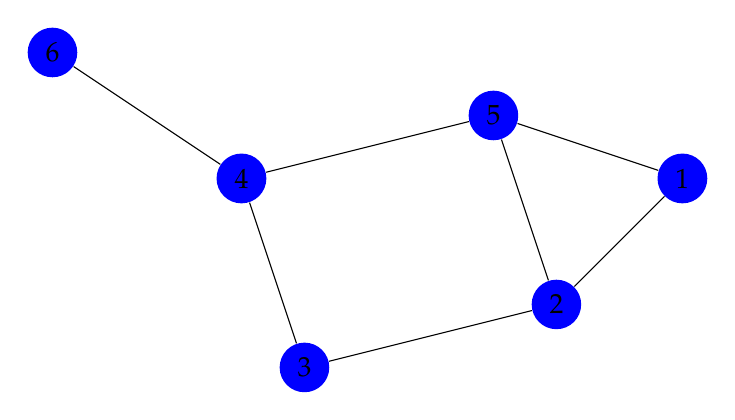
\begin{tikzpicture}
		[scale=0.8,auto=left,every node/.style={circle,fill=blue!100}]
		\node (n6) at (1,10) {6};
		\node (n4) at (4,8)  {4};
		\node (n5) at (8,9)  {5};
		\node (n1) at (11,8) {1};
		\node (n2) at (9,6)  {2};
		\node (n3) at (5,5)  {3};
		
		\foreach \from/\to in {n6/n4,n4/n5,n5/n1,n1/n2,n2/n5,n2/n3,n3/n4}
		\draw (\from) -- (\to); 
		\end{tikzpicture}
	\end{center}
	
\end{enumerate}



\subsection{Creating tables}
Here we show some simple examples of writing table in \LaTeX\. For more complicated tables, according to your requirements, 
you can see the following page: \\
\noindent 
\href{https://www.overleaf.com/learn/latex/Tables}{https://www.overleaf.com/learn/latex/Tables}. 

\begin{table}[h!]
	\centering
		\begin{tabular}{|c|c|c|c|}
		\hline % draw a horizontal line. 
		1 & A & B & C \\ 
		\hline
		2 & D & E & F \\ 
		\hline
		3 & G & H & I \\ 
		\hline
	\end{tabular}
	\caption{Simple Table}
	\label{table:0}
\end{table}

\noindent
Here is an example of two tables placed side by side. 
\begin{table}[h!] % To place the table at this precise location, use the parameter h!. 
\parbox{.45\linewidth}{
\centering 
	\begin{tabular}{|c|c|c|c|}
		\hline
		\multicolumn{4}{|c|}{Sample space 1} \\ 
		\hline
		1 & A & B & C \\ 
		\hline
		2 & D & E & F \\ 
		\hline
		3 & G & H & I \\ 
		\hline
	\end{tabular}
	\caption{List of items 1}
	\label{table:1}
}
\hfill
\parbox{.45\linewidth}{
\centering 
\begin{tabular}{|c|c|c|c|}
	\hline
	\multicolumn{4}{|c|}{Sample space 2} \\ 
	\hline
	1 & A & B & C \\ 
	\hline
	2 & D & E & F \\ 
	\hline
	3 & G & H & I \\ 
	\hline
\end{tabular}
\caption{List of items 2}
\label{table:2}
}
\end{table}


\newpage 
\section{Acknowledgements}
\small{The authors would like to thank ``Name Surname'' for useful discussions. 
The first named author is supported by ``name of funding agency''. } 



\pdfbookmark[-1]{Reference}{thebibliography}
%\addcontentsline{toc}{chapter}{Reference}
\begin{thebibliography}{AA}
	\providecommand{\doi}[2][]{doi: \href{https://doi.org/#2}{#2}}
	\providecommand{\arxiv}[2][]{arXiv:\href{https://arxiv.org/abs/#2}{#2}} 
	
	\bibitem{Atiyah-1957}
	M. F. Atiyah, Complex analytic connections in fibre bundles, 
	\textit{Trans. Amer. Math. Soc.}, \textbf{85} (1957), 181--207. 
	\doi{10.2307/1992969}. 
	
	\bibitem{Deligne-1970}
	Pierre Deligne, \textit{\'Equations diff\'erentielles \`a points singuliers r\'eguliers}, 
	Lecture Notes in Mathematics, Vol. 163, Springer-Verlag, Berlin-New York (1970). 
	\doi{10.1007/BFb0061194}. 
	
	\bibitem{Hartshorne-1977}
	Robin Hartshorne, \textit{Algebraic geometry}, Graduate Texts in Mathematics, No. 52. 
	\textit{Springer-Verlag, New York-Heidelberg}, 1977.  
	\doi{10.1007/978-1-4757-3849-0}. 
	
	\bibitem{Voisin-I}
	Claire Voisin, \textit{Hodge theory and complex algebraic geometry. I}, 
	\textit{Cambridge Studies in Advanced Mathematics}, volume~76, 
	Cambridge University Press, Cambridge, english edition (2007). 
	\doi{10.1017/CBO9780511615344}. 
	
	\bibitem{Weil-1938}
	Andr\'e Weil, Généralisation des fonctions abéliennes, 
	\textit{J. Math. Pures Appl.}, \textbf{17} (1938), 47--87. 
\end{thebibliography}
%}

\end{document}